\section{Problem Setup}

We assume a set of communicating components (i.e., actors, or \Code{P}
machines) that interact with each other asynchronously. These
components may model an application that implements a distributed
protocol over a set of processes or describe some external entity
available to the application (e.g., a storage system or database).
Each component is equipped with a specification that governs its
allowed behaviors.  We formalize these specifications using the same
language we used in our PLDI'24 paper (i.e., LTL$_f$) that has a
natural representation as symbolic finite automata (SFA).  We have
refined our specification language so that they are now additionally
equipped with predicates that model the system's overall asynchronous
semantics.  For example, a read request performed by a client
component may not necessarily be immediately serviced by the server
components.

\paragraph{Axioms and Specification} As a result of the inherently
asynchronous semantics of the systems we're modeling, component
specifications must capture how one message (aka event) might trigger
another. For instance, a specification that is associated with a
coordinator that manages a 2PC protocol using a backing database as a
persistent store might capture the property that a read request that
it receives initiates a chain of additional events or messages as
follows:
\begin{align*}
    \eff{ReadReq} \to \eff{GetReq} \to \eff{GetRsp}(v) \to
    \eff{ReadRsp}(v)
\end{align*}
\noindent where the payload of both $\eff{GetRsp}$ and $\eff{ReadRsp}$
contains the same value. These relationships are referred to as axioms
and are represented as individual temporal specifications for each
kind of message handled by components. For example, the specification
$\phi_{\eff{ReadReq}}$ defined above specifies that when the
coordinator handles a $\eff{ReadReq}$, it will send a $\eff{GetReq}$
to the database.

The LTL$_f$ specifications for a 2PC coordinator and all participating
processes can be mechanically extracted from their corresponding
\Code{P} implementations. For example, the relation between
$\eff{GetRsp}$ and $\eff{ReadRsp}$ shown above can be automatically
extracted from the following \Code{P} code.

\begin{minted}[xleftmargin=5pt, numbersep=4pt, linenos = true, fontsize = \footnotesize, escapeinside=??]{C}
on GetRsp do (input: ...) {
    /* code that handles read request is omitted */
    
    // handler always ends up with message sending
    send client, ReadRsp, (v = input.v,); // feild v of ReadReq's payload is equal to GetReq's
}
\end{minted}


\paragraph{Problem Setting}

Our tool takes a set of axioms $\Phi$ as described above and a
correctness property $A$ as input, and \emph{synthesizes} a program
$P$ that simulates a full test environment, generating requests to the
server (i.e., program under test), handling responses, and defining a
linearizable schedule among the components comprising the system.  By
removing ordering constraints on message communication among
components that are explicit in the synthesized program, we instead
get a specification-driven client (test generator) that relies on an external
scheduler, similar to the existing setup that uses the native
$\Code{P}$ scheduler and monitor to manage interaction between
components.

\section{Motivating Example}

\begin{figure}[ht!]
    \centering
    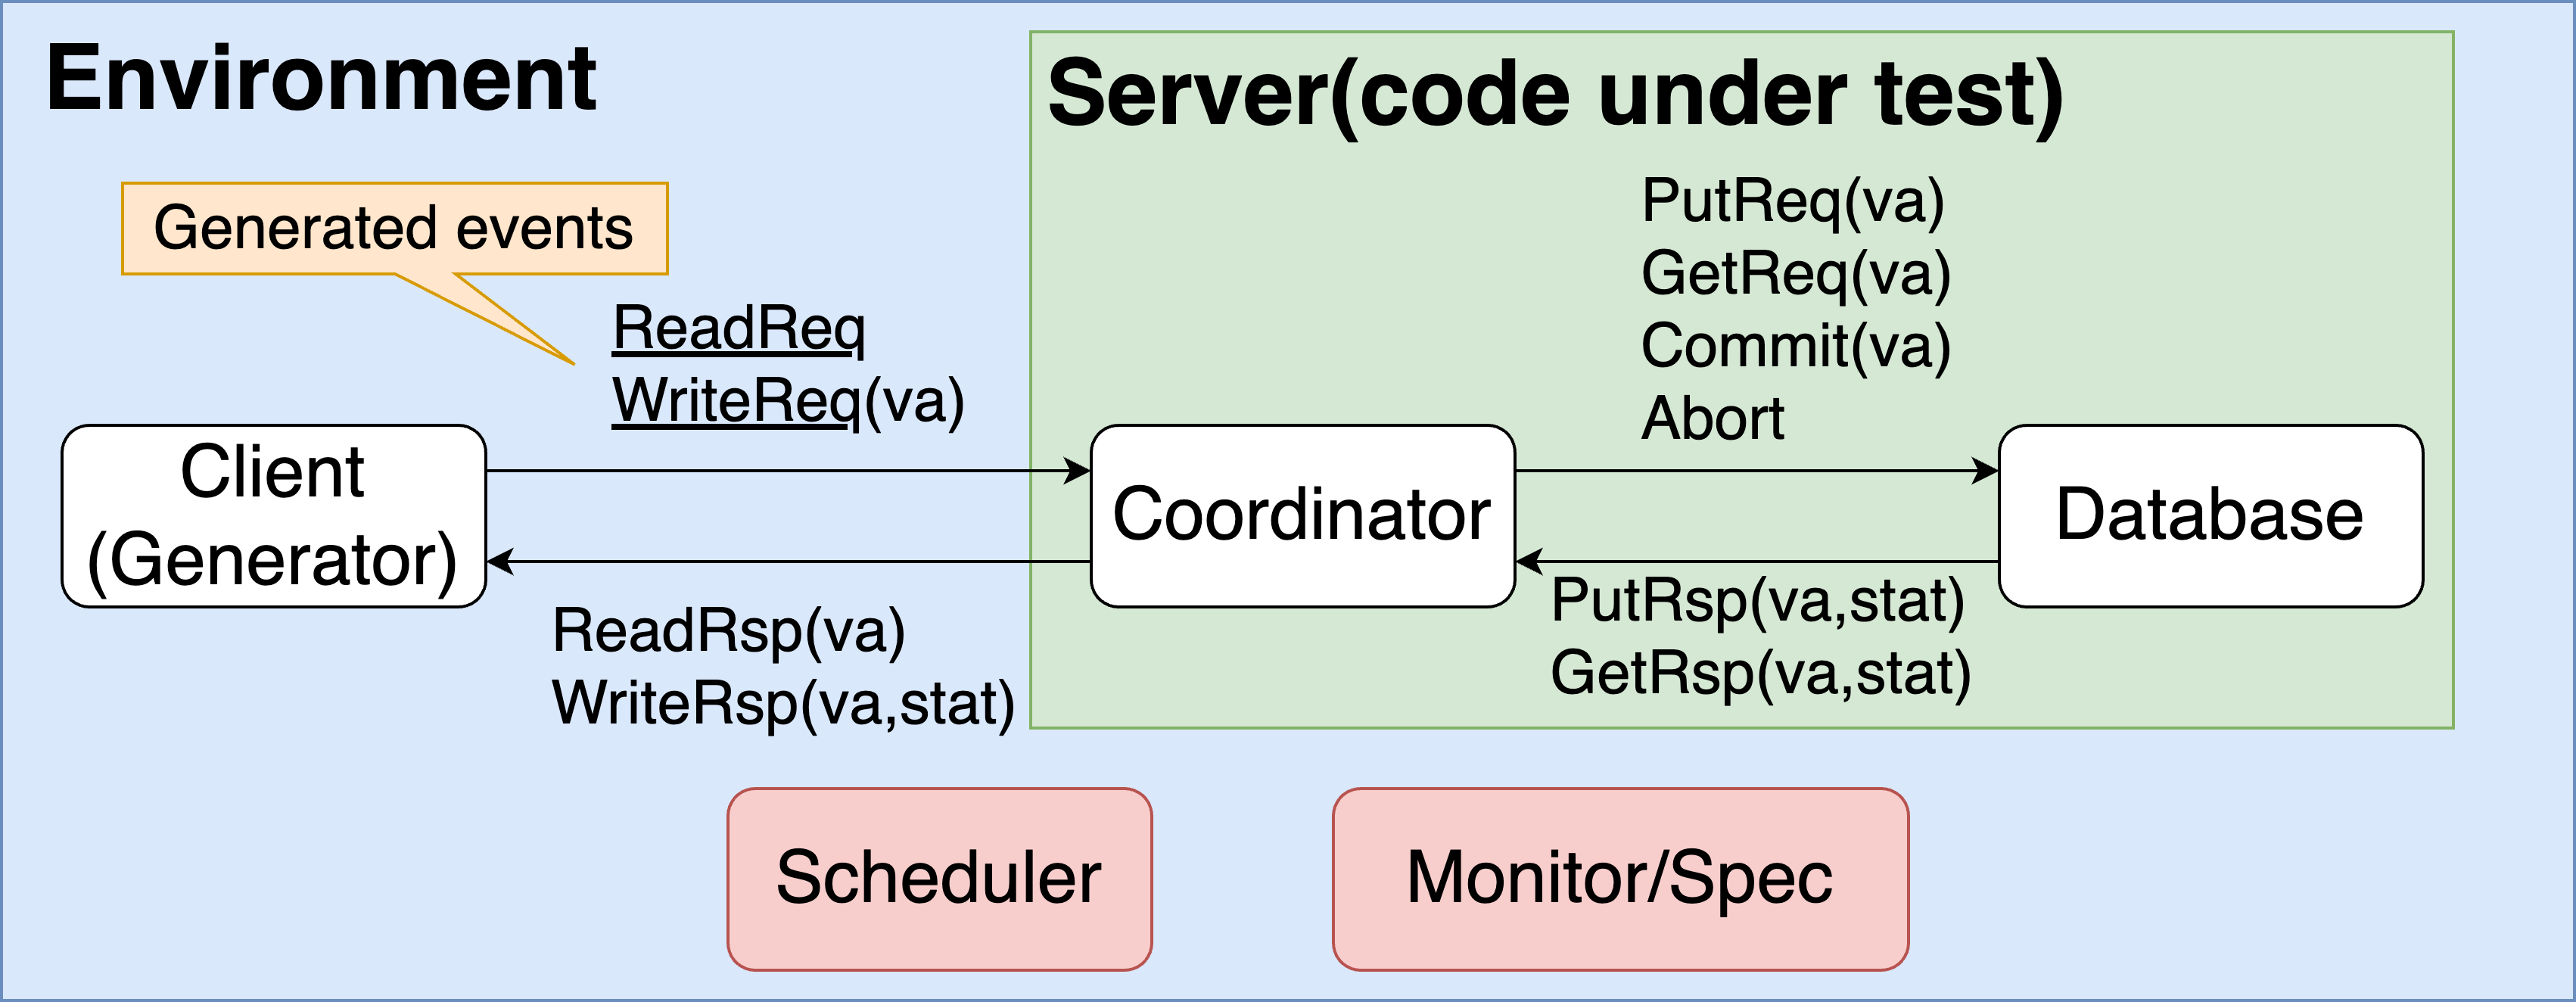
\includegraphics[width=0.75\linewidth]{figures/typed-guided-planing-example.drawio.png}
    \caption{A simplified two-phase commit model.}
    \label{fig:ex-2pc}
\end{figure}

Following the above, we present a simplified two-phase commit model to
motivate our approach, as depicted in \autoref{fig:ex-2pc}. This model
comprises four components (\Code{P} machines):
\begin{enumerate} 
    \item The client (generator) simulates user behaviors, enabling the sending
      and receiving of $\eff{Read/Write}$ messages for reading and
      writing values (specifically, the field $\Code{v}$ in the
      payloads). Furthermore, the response message (i.e., messages end
      with $\eff{Rsp}$) includes a Boolean field, $\Code{stat}$, which
      indicates the status code of the action performed.  
    \item The code under test (server), illustrated in green in
      \autoref{fig:ex-2pc}, consists of two types of components: the
      coordinator and the database. For clarity, we refer to
      the interactions between the coordinator and the database using
      $\eff{Put/Get}$ instead of read/write. The actual data is stored
      within the database component, while the coordinator retrieves
      this data and determines whether the updated information should
      be made persistent through $\eff{Commit}$ or $\eff{Abort}$
      messages.
    \item A scheduler determines the specific receiving ordering of messages
      sent and received by components.
    \item A monitor that determines that messages observed by the
      coordinator and database are consistent with a global
      correctness property.
\end{enumerate}


\paragraph{Correctness Property} We aim to establish a correctness property $\exArw$,
which, for this example, asserts that strong consistency is preserved.\\[-.8em]

$\exArw$: \textit{Any read result (i.e., the $\Code{v}$ field of
  $\eff{ReadRsp}$) must equal the most recent successfully written
  value (i.e., when the $\Code{stat}$ field of $\eff{WriteRsp}$ is
  \Code{true}).}\\[-.8em]

The correctness property $\exArw$ can be formulated as a symbolic LTL
(Linear Temporal Logic) formula. However, the implementation may not
align with its requirements. For instance, the specifications
associated with database may only guarantee eventual consistency;
thus, a read result immediately following a successful committed write
might not reflect the written value, as the database may process the
read request logically out-of-order with the $\eff{Commit}$ message.

\paragraph{Environment and Generator} The environment encompasses
the elements required by the program under test (i.e., the
coordinator and database) during execution.  Our tool synthesizes
a program that models the behavior of the environment.  The behaviors
exhibited by this program are guaranteed to be consistent with
the specifications associated with the components being tested.

An important element of the environment is a generator that produces
\emph{generated events} (e.g., $\eff{WriteReq}$ and $\eff{ReadReq}$)
that need to be handled by the client program. The environment also
includes a scheduler that governs the order in which messages are
received by the actors comprising the coordinator, as well as a
monitor that check whether the \emph{observed} events are consistent
with the correctness property $\exArw$.

Although there are potentially infinitely many environment programs
that can be generated, we are particularly interested in identifying
those that result in the execution of the program under test to
violate the correctness property $\exArw$. This can occur when a
$\eff{ReadReq}$ message is generated after previous issued $\eff{WriteReq}$, which in turn precedes a generated
$\eff{Commit}$ message by the coordinator, but whose return value
payload does not match the payload of the $\eff{WriteReq}$.  An
example of a program that manifests this behavior, denoted as $e$, is
provided below. For simplicity, we assume there is only one
coordinator and one database, and therefore the source and destination
components (\Code{P} machines) of the messages are omitted.

\begin{minted}[xleftmargin=5pt, numbersep=4pt, linenos = true, fontsize = \footnotesize, escapeinside=??]{OCaml}
let (x: int);
?$\mykw{assume}$? (x != -1);
?$\mykw{generate}$? WriteReq x;
(* let (y1: int) = ?$\mykwCmt{observe}$? PutReq; *)
(* ?$\mykwCmt{assume}$? (y1 == x); *)
(* let (y2: int), (s1: bool) = ?$\mykwCmt{observe}$? PutRsp; *)
(* ?$\mykwCmt{assume}$? (y2 == x && s1 == true); *)
let (y3: int), (s2: bool) = ?$\mykw{observe}$? WriteRsp;
(* ?$\mykwCmt{assume}$? (y3 == x && s2 == true); *)
?$\mykw{generate}$? ReadReq;
(* let () = ?$\mykwCmt{observe}$? GetReq; *)
(* let (y4: int) = ?$\mykwCmt{observe}$? GetRsp; *)
(* ?$\mykwCmt{assume}$? (y4 == -1); *)
(* let () = ?$\mykwCmt{observe}$? Commit; *)
let (y5: int) = ?$\mykw{observe}$? ReadRsp;
(* ?$\mykwCmt{assume}$? (y5 == y4 && y5 != x); *)
\end{minted}
This program can be considered as playing three distinct roles, corresponding
to the three distinct elements that make up an environment: as a
generator, a scheduler, and a monitor. Without the commented code, $e$
acts as a generator that sends messages to the coordinator (on lines
$3$ and $10$) and receive responses (on lines $10$ and $15$). This
behavior is analogous to the following \Code{P} code.

\begin{minted}[xleftmargin=5pt, numbersep=4pt, linenos = true, fontsize = \footnotesize, escapeinside=??]{C}
var x: int;
while (x != -1) {
    x = choose(int);
}
send coordinator, WriteReq, (source = this, v = x);
receive {
    case WriteRsp: ((y3: int, s2: bool)) {}
}
send coordinator, ReadReq, (source = this,);
receive {
    case ReadRsp: ((y5: int,)) {}
}
\end{minted}

\noindent We distinguish messages sent by the generator from other
messages. The former are ``announced'' using the $\mykw{generate}$
keyword, and it is the responsibility of the execution environment in
which this program runs to provide the concrete payload of the
message.  On the other hand, the environment can also $\mykw{observe}$
other messages and store the corresponding payload into variables
(e.g., $y_3$ on line $8$).

The synthesized program, without the commented code, can be naturally
integrated with the native $\Code{P}$ framework.  However, if we
include the commented code, the program gains a global view (i.e.,
visibility of all events) and additionally functions as a scheduler,
dictating the order in which messages are received.  For instance, the
$\eff{Commit}$ message (line $14$) is received after the
$\eff{GetRsp}$ message (line $12$), which is why the read value
remains the default value (i.e., $-1$) rather than the value that was
successfully written.  It's important to note that, aside from
scheduling, the behaviors of components can also be
non-deterministic. For example, the database might send a
$\eff{WriteRsp}$ with a $\false$ status (line $9$). In this context,
the $\mykw{assume}$ keyword in the commented code acts as a monitor,
ensuring that the execution indeed produces a trace that violates the
correctness property $\exArw$.

Because specifications for these components are overapproximate,
however, it is not guaranteed that even in this elaborated version,
the set of provided responses to a messages will lead to a violation
of the correctness property; for example, the \Code{assume} statement
on Line (7) may fail since the \Code{PutResp} on Line 6 is not assured
to always return true.  However, we can ensure that there is \emph{some}
consistent assignment to these variables that satisfies all
\Code{assume} statements and leads the execution to a violation of the
correctness property.

\paragraph{Why our approach works}  Our underlying intuition is that
having such a ``global view'' that assembles an execution from local
component interactions based on specification constraints can can lead
to a more effective and directed testing strategy. Therefore, we first
synthesize an environment that acts as both a generator and a
scheduler. Even if we later ``erase'' those messages that are not sent
or received by the generator, the testing procedure remains more
efficient since the sequence of inputs produced by the generator are
specification driven.

Additionally, we can optimize the ``guess and filter'' loop found on
lines $1$ to $4$ of the analogous \Code{P} code shown earlier by
implementing a more efficient approach. This can be achieved by
repeatedly querying an SMT solver (e.g., $\Code{z3}$) to provide
different values that satisfy the $\mykw{assume}$ constraint (e.g., $x
\not= -1$). This approach is especially useful when dealing with
complex constraints.

\section{Progress and Plan}

We have recently adapted our prior work from PLDI '24 to formalize
this problem as a deductive synthesis task. Similar to other deductive
synthesis approaches, we have defined a set of declarative derivation
rules as the theoretical foundation, ensuring soundness for our
approach.

However, during deductive synthesis, there are often multiple
applicable declarative rules, and only by selecting the appropriate
ones can we successfully derive a correctly synthesized program. This
selection process involves non-trivial searching in a large search
space of possible rule application orders. To address this challenge,
we are designing a synthesis algorithm that applies these rules in a
more deterministic and efficient manner. This algorithm will
essentially formalize the heuristic strategies developed during the
previous internship.

Our goal is to complete this algorithm by mid-October, leaving us with
about a month before PLDI's submission deadline (November 14th) to run
experiments and finalize the paper.
